\documentclass[12pt,letterpaper]{article}
\usepackage[utf8]{inputenc}
\usepackage[spanish]{babel}
\usepackage{graphicx}
\usepackage[hidelinks]{hyperref}
\usepackage{hyperref}
\usepackage[left=2cm,right=2cm,top=2.5cm,bottom=2cm]{geometry}
\usepackage{graphicx} % figuras
\usepackage{float} % para usar [H]
\usepackage{amsmath}
\usepackage{stackrel} 
\usepackage{multicol}
\usepackage{multirow}
\usepackage{fancyhdr}
\usepackage[usenames,dvipsnames,svgnames,table]{xcolor}
\usepackage[document]{ragged2e}
\usepackage{enumerate} % enumerados
\renewcommand{\labelitemi}{$-$}
\renewcommand{\labelitemii}{$\cdot$}
\newcommand\tab[1][1cm]{\hspace*{#1}}

\definecolor{amarillo}{RGB}{255,255,0}
\definecolor{rojo}{RGB}{255,0,0}
\definecolor{azul}{RGB}{0,0,255}
\definecolor{verdeClaro}{RGB}{0,255,0}

%encabezado
\pagestyle{fancy}
\lhead{\begin{picture}(0,0) \put(0,0){
\includegraphics[width=10mm]{./img/logo}} \end{picture}}
\chead{\hspace{1cm}\vspace{0.2cm}INFORME DE LABORATORIO N° 05 - ELABORACION DE REPORTES OPERACIONALES}
\rhead{}

\begin{document}
    \begin{titlepage}
        \begin{center}
            \begin{figure}[htb]
                \begin{center}
                    
\includegraphics[width=3.5cm]{./img/logo}
                \end{center}
            \end{figure}
            \vspace*{0.15in}
            \begin{Large}
                \textbf{UNIVERSIDAD PRIVADA DE TACNA}\\
            \end{Large}
            \vspace*{0.15in}
            \begin{Large}
                \textbf{FACULTAD DE INGENIERIA} \\
            \end{Large}
            \vspace*{0.1in}
            \begin{Large}
                \textbf{Escuela Profesional de Ingeniería de Sistemas} \\
            \end{Large}
            \vspace*{0.3in}
            \begin{Large}
                \textbf{INFORME DE LABORATORIO N°05}\\
                \textbf{``ELABORACION DE REPORTES OPERACIONALES"}\\
            \end{Large}
            \vspace*{0.2in}
            \begin{Large}
                \textbf{CURSO:} \\
            \end{Large}
            \vspace*{0.1in}
            \begin{large}
                Inteligencia de Negocios\\
            \end{large}
            \vspace*{0.2in}
            \begin{Large}
                \textbf{DOCENTE:} \\
            \end{Large}
            \vspace*{0.1in}
            \begin{large}
                Mag. Patrick Jose Cuadros Quiroga\\
            \end{large}
            \vspace*{0.3in}
            \begin{large}
                \textbf{ALUMNO:} \\
                \begin{flushleft}
                    Gutierrez Ponce, José Carlos  		\hfill	(2017059277) \\
                \end{flushleft}
            \end{large}
            \vspace*{1.3in}
            \begin{large}
                Tacna - Perú\\
            \end{large}
            \vspace*{0.1in}
            \begin{large}
                2021\\
            \end{large}
        \end{center}
    \end{titlepage}
    \include{Secciones/articulo}
    %%%%%%%%%%%%%%%%%%%%%%%%%%%%%%%%%%%%%%%%%%%%%%%%%%%%%%%%%%%%%%%%%%%%%%%%%%%%%%%%%%%%%%%%%%%%%%%%%%%%%%%%%%%%%%%%%%%%%%%%%%%%%%%%%%%%%%%%%%%%%%%%%%%%%%%%%%%%%%%%%%%%%%%%%%%%%%%%%%%%%%%%%%%%%%%%%%%%%%%%%%%%%%%%%%%%%%%%%%%%%%%%%%%%%%%%%%%%%%%%%%%%%%%%%%%%%%%%%%%%%%%%%%%%%%%%%%%%%%%%%%%%%%%%%%%%%%%%%%%%%%%%%%%%%%%%%%%%%%%%%%%%%%%%%%%%%%%%%%%%%%%%%%%%%%%%%%%%%%%%%%%%%%%%%%%%%%%%%%%%%%%%%%%%%%%%%%%%%%%%%%%%%%%%%%%%%%%%%%%%%%%%%%%%%%%%%%%%%%%%%%%%%%%%%%%%%%%%%%%%%%%%%%%%%%%%%%%%%%%%%%%%%%%%%%%%%%%
    \newpage
    \tableofcontents
    \justify
    %%%%%%%%%%%%%%%%%%%%%%%%%%%%%%%%%%%%%%%%%%%%%%%%%%%%%%%%%%%%%%%%%%%%%%%%%%%%%%%%%%%%%%%%%%%%%%%%%%%%%%%%%%%%%%%%%%%%%%%%%%%%%%%%%%%%%%%%%%%%%%%%%%%%%%%%%%%%%%%%%%%%%%%%%%%%%%%%%%%%%%%%%%%%%%%%%%%%%%%%%%%%%%%%%%%%%%%%%%%%%%%%%%%%%%%%%%%%%%%%%%%%%%%%%%%%%%%%%%%%%%%%%%%%%%%%%%%%%%%%%%%%%%%%%%%%%%%%%%%%%%%%%%%%%%%%%%%%%%%%%%%%%%%%%%%%%%%%%%%%%%%%%%%%%%%%%%%%%%%%%%%%%%%%%%%%%%%%%%%%%%%%%%%%%%%%%%%%%%%%%%%%%%%%%%%%%%%%%%%%%%%%%%%%%%%%%%%%%%%%%%%%%%%%%%%%%%%%%%%%%%%%%%%%%%%%%%%%%%%%%%%%%%%%%%%%%%%
    \newpage
    \begin{LARGE}
        \begin{center}
            \textbf{ELABORACION DE REPORTES OPERACIONALES}\\
        \end{center}
    \end{LARGE}
    %%%%%%%%%%%%%%%%%%%%%%%%%%%%%%%%%%%%%%%%%%%%%%%%%%%%%%%%%%%%%%%%%%%%%%%%%%%%%%%%%%%%%%%%%%%%%%%%%%%%%%%%%%%%%%%%%%%%%%%%%%%%%%%%%%%%%%%%%%%%%%%%%%%%%%%%%%%%%%%%%%%%%%%%%%%%%%%%%%%%%%%%%%%%%%%%%%%%%%%%%%%%%%%%%%%%%%%%%%%%%%%%%%%%%%%%%%%%%%%%%%%%%%%%%%%%%%%%%%%%%%%%%%%%%%%%%%%%%%%%%%%%%%%%%%%%%%%%%%%%%%%%%%%%%%%%%%%%%%%%%%%%%%%%%%%%%%%%%%%%%%%%%%%%%%%%%%%%%%%%%%%%%%%%%%%%%%%%%%%%%%%%%%%%%%%%%%%%%%%%%%%%%%%%%%%%%%%%%%%%%%%%%%%%%%%%%%%%%%%%%%%%%%%%%%%%%%%%%%%%%%%%%%%%%%%%%%%%%%%%%%%%%%%%%%%%%%%
    \section{OBJETIVOS}
    \begin{itemize}
        \item Crear reportes operacionales a partir de una BD SQL con una herramienta de visualizacion de BI.
    \end{itemize}
    %%%%%%%%%%%%%%%%%%%%%%%%%%%%%%%%%%%%%%%%%%%%%%%%%%%%%%%%%%%%%%%%%%%%%%%%%%%%%%%%%%%%%%%%%%%%%%%%%%%%%%%%%%%%%%%%%%%%%%%%%%%%%%%%%%%%%%%%%%%%%%%%%%%%%%%%%%%%%%%%%%%%%%%%%%%%%%%%%%%%%%%%%%%%%%%%%%%%%%%%%%%%%%%%%%%%%%%%%%%%%%%%%%%%%%%%%%%%%%%%%%%%%%%%%%%%%%%%%%%%%%%%%%%%%%%%%%%%%%%%%%%%%%%%%%%%%%%%%%%%%%%%%%%%%%%%%%%%%%%%%%%%%%%%%%%%%%%%%%%%%%%%%%%%%%%%%%%%%%%%%%%%%%%%%%%%%%%%%%%%%%%%%%%%%%%%%%%%%%%%%%%%%%%%%%%%%%%%%%%%%%%%%%%%%%%%%%%%%%%%%%%%%%%%%%%%%%%%%%%%%%%%%%%%%%%%%%%%%%%%%%%%%%%%%%%%%%%
    \section{REQUERIMIENTOS}
    \begin{itemize}
        \item Conocimientos\\
        Para el desarrollo de esta práctica se requerirá de los siguientes conocimientos básicos:
        \begin{itemize} 
            \item Conocimientos básicos de administración de base de datos Microsoft SQL Server.
            \item Conocimientos básicos de SQL.
        \end{itemize}
        \item Hardware
        \begin{itemize}
            \item CPU SLAT-capable feature.
            \item Al menos 4GB de RAM.
        \end{itemize}
        \item Software\\
        Así mismo se necesitan los siguientes aplicativos
        \begin{itemize}
            \item WMicrosoft SQL Server 2017 o superior.
        \end{itemize}
    \end{itemize}
    %%%%%%%%%%%%%%%%%%%%%%%%%%%%%%%%%%%%%%%%%%%%%%%%%%%%%%%%%%%%%%%%%%%%%%%%%%%%%%%%%%%%%%%%%%%%%%%%%%%%%%%%%%%%%%%%%%%%%%%%%%%%%%%%%%%%%%%%%%%%%%%%%%%%%%%%%%%%%%%%%%%%%%%%%%%%%%%%%%%%%%%%%%%%%%%%%%%%%%%%%%%%%%%%%%%%%%%%%%%%%%%%%%%%%%%%%%%%%%%%%%%%%%%%%%%%%%%%%%%%%%%%%%%%%%%%%%%%%%%%%%%%%%%%%%%%%%%%%%%%%%%%%%%%%%%%%%%%%%%%%%%%%%%%%%%%%%%%%%%%%%%%%%%%%%%%%%%%%%%%%%%%%%%%%%%%%%%%%%%%%%%%%%%%%%%%%%%%%%%%%%%%%%%%%%%%%%%%%%%%%%%%%%%%%%%%%%%%%%%%%%%%%%%%%%%%%%%%%%%%%%%%%%%%%%%%%%%%%%%%%%%%%%%%%%%%%%%
    \newpage
    \section{DESARROLLO}
    \subsection{Parte I: Crear BD}
    \begin{enumerate}[\tab 1.]
        \item Debe crear la base de datos con el nombre \textbf{Control\_de\_libros\_Sucarnet}, tomando en cuenta las relaciones entre las tablas (llaves primarias y llaves foráneas). Así como se presenta en la siguiente figura:\\[0.1in]
        \begin{center}
            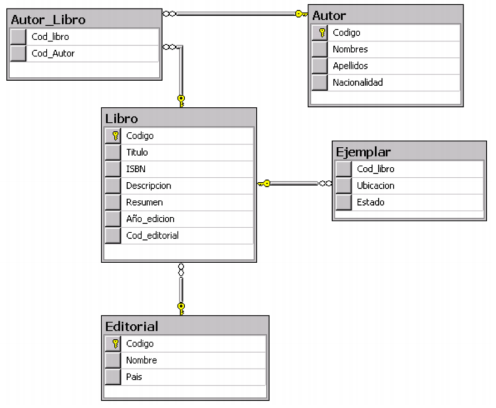
\includegraphics[width=13cm]{./img/img1.png}
        \end{center}
        \begin{itemize}
            \item Creamos la \textbf{BD} usando el siguiente comando:
            \begin{center}
                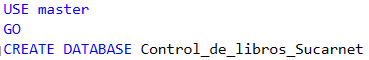
\includegraphics[width=13cm]{./img/img1.1.png}
            \end{center}
            \item Creamos la tabla \textbf{Autor} usando el siguiente comando:
            \begin{center}
                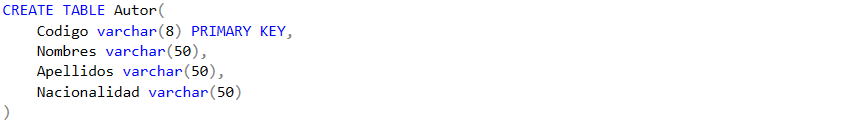
\includegraphics[width=13cm]{./img/img1.2.png}
            \end{center}
            \item Creamos la tabla \textbf{Editorial} usando el siguiente comando:
            \begin{center}
                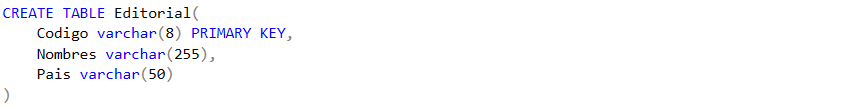
\includegraphics[width=13cm]{./img/img1.3.png}
            \end{center}
            \item Creamos la tabla \textbf{Libro} usando el siguiente comando:
            \begin{center}
                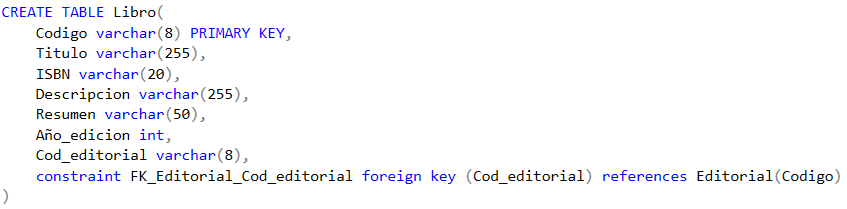
\includegraphics[width=13cm]{./img/img1.4.png}
            \end{center}
            \item Creamos la tabla \textbf{Ejemplar} usando el siguiente comando:
            \begin{center}
                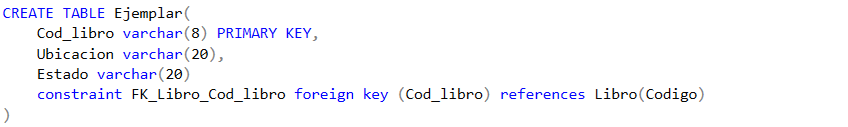
\includegraphics[width=13cm]{./img/img1.5.png}
            \end{center}
            \item Creamos la tabla \textbf{Autor\_Libro} usando el siguiente comando:
            \begin{center}
                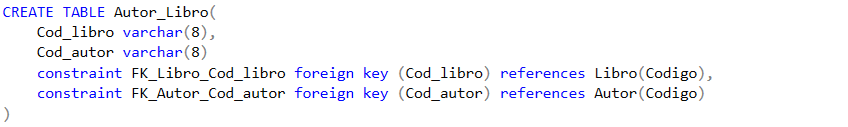
\includegraphics[width=13cm]{./img/img1.6.png}
            \end{center}
        \end{itemize}
        \item Agregar los siguientes datos a cada tabla.
        \begin{itemize}
            \item Tabla Autor.s
            \begin{center}
                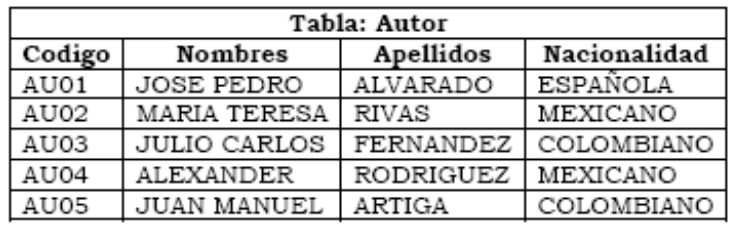
\includegraphics[width=13cm]{./img/img2.png}
            \end{center}
            Para agregar los datos usar el siguiente codigo:
            \begin{center}
                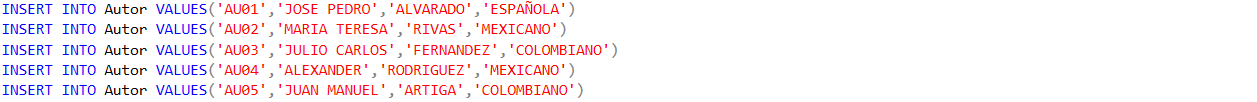
\includegraphics[width=13cm]{./img/img2.1.png}
            \end{center}
            \item Tabla Editorial.
            \begin{center}
                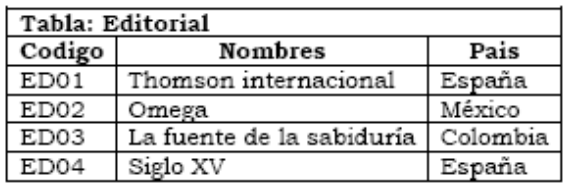
\includegraphics[width=13cm]{./img/img3.png}
            \end{center}
            Para agregar los datos usar el siguiente codigo:
            \begin{center}
                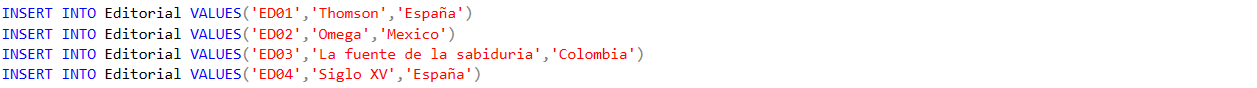
\includegraphics[width=13cm]{./img/img3.1.png}
            \end{center}
            \item Tabla Libro.
            \begin{center}
                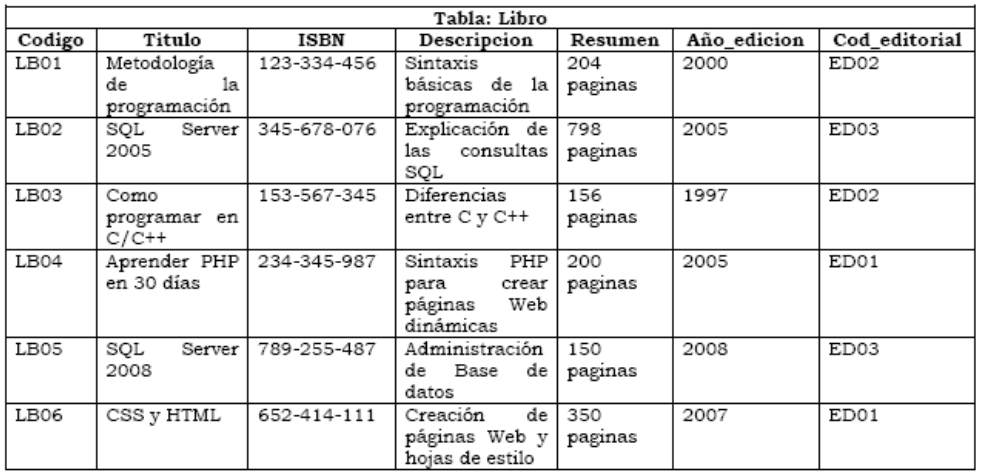
\includegraphics[width=13cm]{./img/img4.png}
            \end{center}
            Para agregar los datos usar el siguiente codigo:
            \begin{center}
                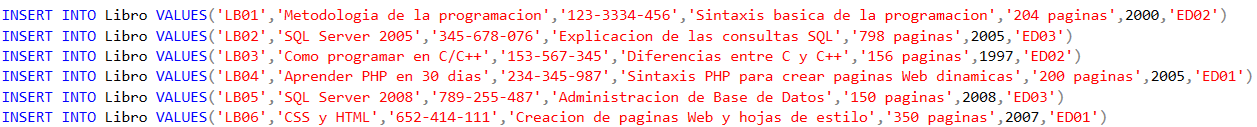
\includegraphics[width=13cm]{./img/img4.1.png}
            \end{center}
            \item Tabla Ejemplar.
            \begin{center}
                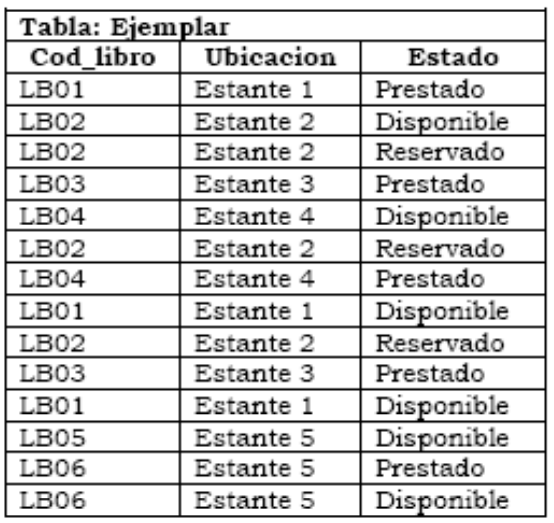
\includegraphics[width=13cm]{./img/img5.png}
            \end{center}
            Para agregar los datos usar el siguiente codigo:
            \begin{center}
                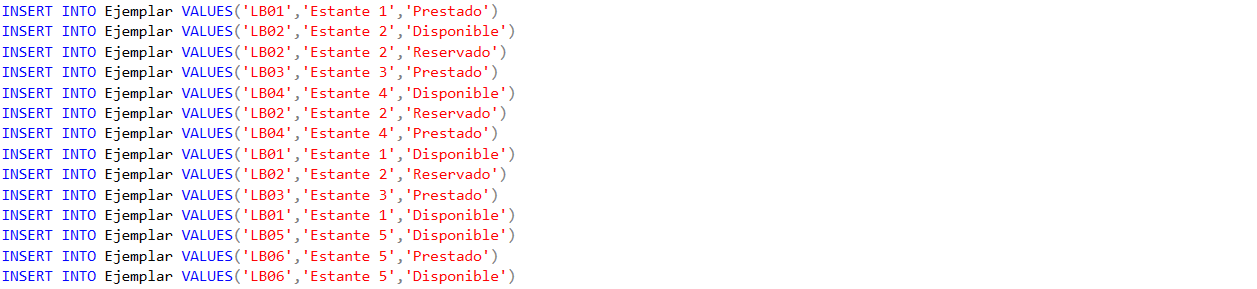
\includegraphics[width=13cm]{./img/img5.1.png}
            \end{center}
            \item Tabla Autor\_Libro.
            \begin{center}
                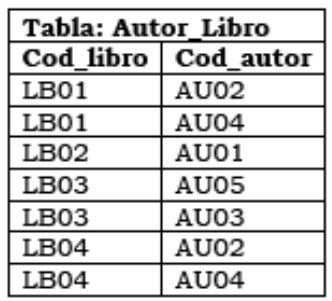
\includegraphics[width=13cm]{./img/img6.png}
            \end{center}
            Para agregar los datos usar el siguiente codigo:
            \begin{center}
                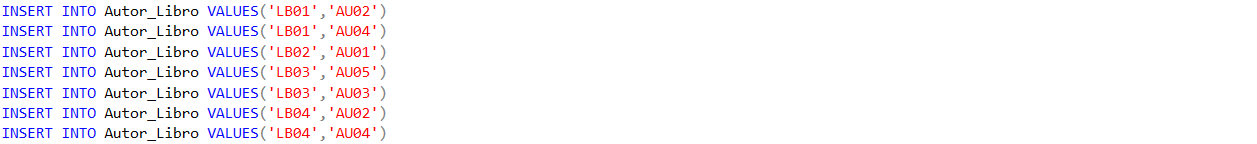
\includegraphics[width=13cm]{./img/img6.1.png}
            \end{center}
        \end{itemize}
    \end{enumerate}
    %%%%%%%%%%%%%%%%%%%%%%%%%%%%%%%%%%%%%%%%%%%%%%%%%%%%%%%%%%%%%%%%%%%%%%%%%%%%%%%%%%%%%%%%%%%%%%%%%%%%%%%%%%%%%%%%%%%%%%%%%%%%%%%%%%%%%%%%%%%%%%%%%%%%%%%%%%%%%%%%%%%%%%%%%%%%%%%%%%%%%%%%%%%%%%%%%%%%%%%%%%%%%%%%%%%%%%%%%%%%%%%%%%%%%%%%%%%%%%%%%%%%%%%%%%%%%%%%%%%%%%%%%%%%%%%%%%%%%%%%%%%%%%%%%%%%%%%%%%%%%%%%%%%%%%%%%%%%%%%%%%%%%%%%%%%%%%%%%%%%%%%%%%%%%%%%%%%%%%%%%%%%%%%%%%%%%%%%%%%%%%%%%%%%%%%%%%%%%%%%%%%%%%%%%%%%%%%%%%%%%%%%%%%%%%%%%%%%%%%%%%%%%%%%%%%%%%%%%%%%%%%%%%%%%%%%%%%%%%%%%%%%%%%%%%%%%%%
    \subsection{Parte II: Crear consultas SQL}
    Utilizando consultas a múltiples tablas resolver los siguientes problemas:
    \begin{enumerate}[\tab 1.]
        \item Se desea mostrar los datos de los autores junto con los títulos de libros que han escrito. Ordenarlos en forma descendente por el nombre del autor\\[0.1in]
        El codigo seria:
        \begin{center}
            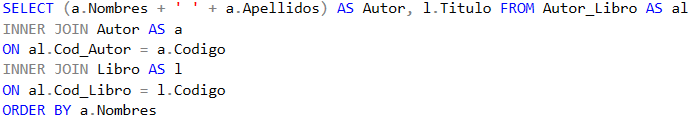
\includegraphics[width=13cm]{./img/img7.1.png}
        \end{center}
        El resultado seria:
        \begin{center}
            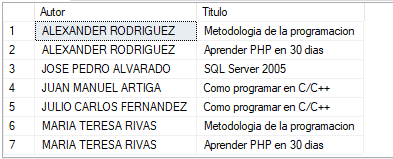
\includegraphics[width=13cm]{./img/img7.2.png}
        \end{center}
        \item Se desea conocer todos los autores que tienen libros que han sido publicados por la editorial “Omega”.\\[0.1in]
        El codigo seria:
        \begin{center}
            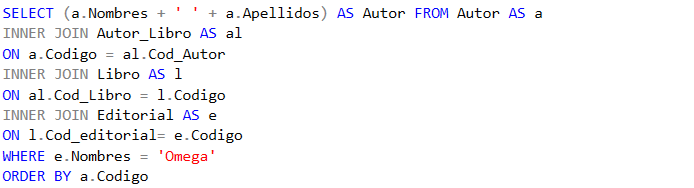
\includegraphics[width=13cm]{./img/img8.1.png}
        \end{center}
        El resultado seria:
        \begin{center}
            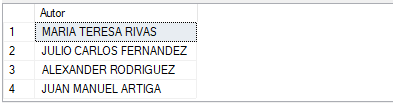
\includegraphics[width=13cm]{./img/img8.2.png}
        \end{center}
        \item Mostrar cuántos ejemplares hay por cada libro. \textbf{Titulo, ejemplar}.\\[0.1in]
        El codigo seria:
        \begin{center}
            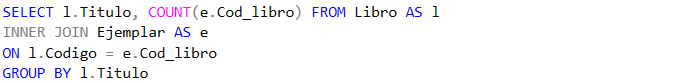
\includegraphics[width=13cm]{./img/img9.1.png}
        \end{center}
        El resultado seria:
        \begin{center}
            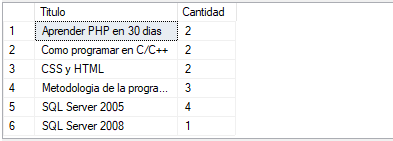
\includegraphics[width=13cm]{./img/img9.2.png}
        \end{center}
        \item Mostrar los \textbf{títulos} de los libros donde el estado sea \textbf{“Prestado”}.\\[0.1in]
        El codigo seria:
        \begin{center}
            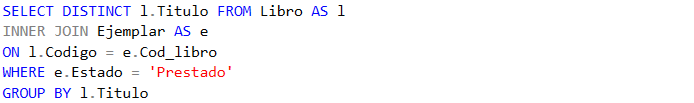
\includegraphics[width=13cm]{./img/img10.1.png}
        \end{center}
        El resultado seria:
        \begin{center}
            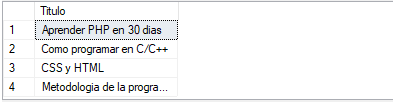
\includegraphics[width=13cm]{./img/img10.2.png}
        \end{center}
        \item Se desea mostrar los libros que se han editados entre el \textbf{2000} y \textbf{2007}. Ordenarlos en forma ascendente.\\[0.1in]
        El codigo seria:
        \begin{center}
            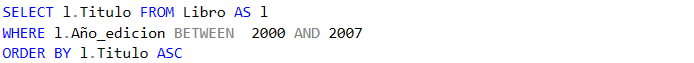
\includegraphics[width=13cm]{./img/img11.1.png}
        \end{center}
        El resultado seria:
        \begin{center}
            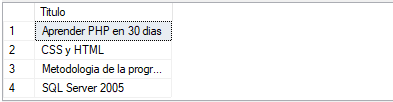
\includegraphics[width=13cm]{./img/img11.2.png}
        \end{center}
        \item Mostrar cuántos libros que se han prestado y agruparlos por el estante\\[0.1in]
        El codigo seria:
        \begin{center}
            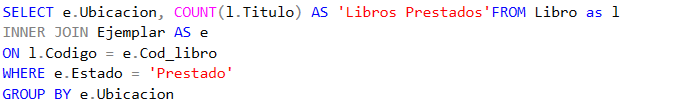
\includegraphics[width=13cm]{./img/img12.1.png}
        \end{center}
        El resultado seria:
        \begin{center}
            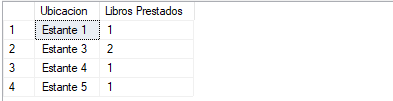
\includegraphics[width=13cm]{./img/img12.2.png}
        \end{center}
    \end{enumerate}
    %%%%%%%%%%%%%%%%%%%%%%%%%%%%%%%%%%%%%%%%%%%%%%%%%%%%%%%%%%%%%%%%%%%%%%%%%%%%%%%%%%%%%%%%%%%%%%%%%%%%%%%%%%%%%%%%%%%%%%%%%%%%%%%%%%%%%%%%%%%%%%%%%%%%%%%%%%%%%%%%%%%%%%%%%%%%%%%%%%%%%%%%%%%%%%%%%%%%%%%%%%%%%%%%%%%%%%%%%%%%%%%%%%%%%%%%%%%%%%%%%%%%%%%%%%%%%%%%%%%%%%%%%%%%%%%%%%%%%%%%%%%%%%%%%%%%%%%%%%%%%%%%%%%%%%%%%%%%%%%%%%%%%%%%%%%%%%%%%%%%%%%%%%%%%%%%%%%%%%%%%%%%%%%%%%%%%%%%%%%%%%%%%%%%%%%%%%%%%%%%%%%%%%%%%%%%%%%%%%%%%%%%%%%%%%%%%%%%%%%%%%%%%%%%%%%%%%%%%%%%%%%%%%%%%%%%%%%%%%%%%%%%%%%%%%%%%%%
    \subsection{Parte III: visualizador}
    Generar reportes operacionales de la parte II utilizando un visualizador Power BI, Tableau o Qlik Sense.
    \begin{enumerate}[\tab 1.]
        \item Se desea mostrar los datos de los autores junto con los títulos de libros que han escrito. Ordenarlos en forma descendente por el nombre del autor
        \begin{center}
            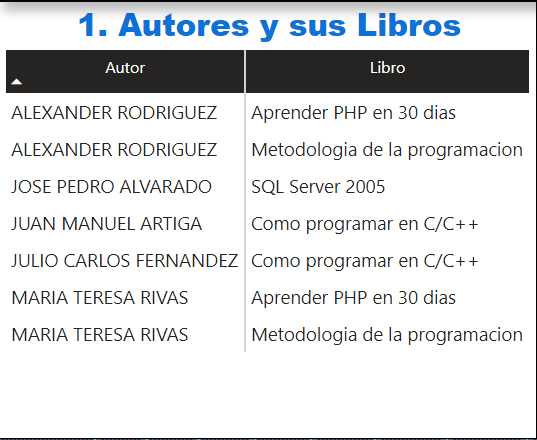
\includegraphics[width=13cm]{./img/img13.png}
        \end{center}
        \item Se desea conocer todos los autores que tienen libros que han sido publicados por la editorial “Omega”.
        \begin{center}
            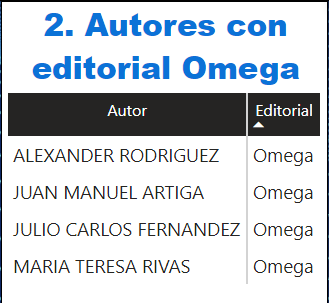
\includegraphics[width=13cm]{./img/img14.png}
        \end{center}
        \item Mostrar cuántos ejemplares hay por cada libro. \textbf{Titulo, ejemplar}.
        \begin{center}
            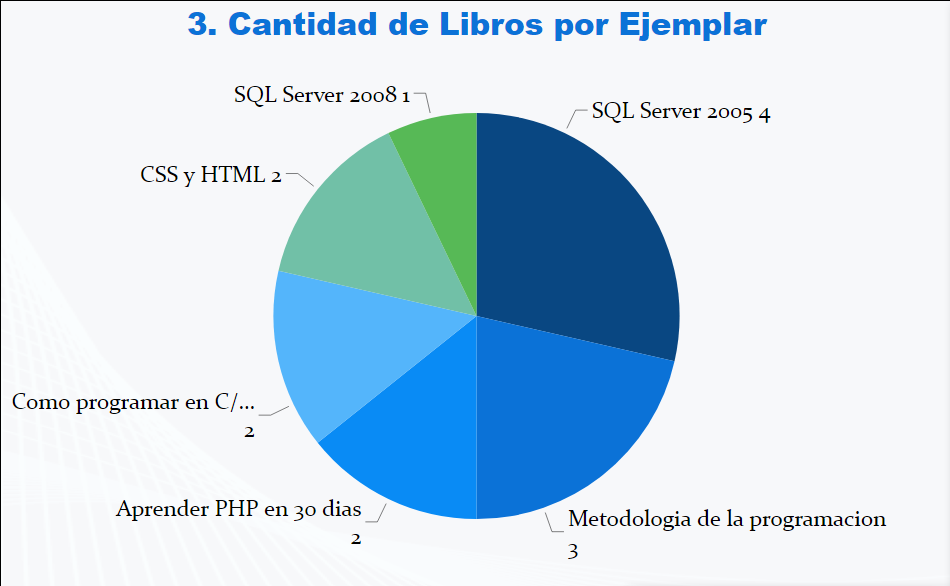
\includegraphics[width=13cm]{./img/img15.png}
        \end{center}
        \item Mostrar los \textbf{títulos} de los libros donde el estado sea \textbf{“Prestado”}.
        \begin{center}
            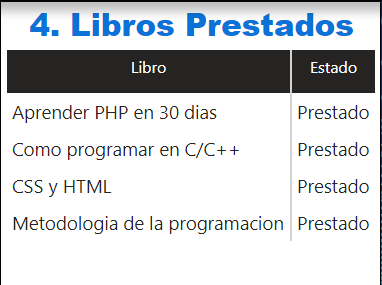
\includegraphics[width=13cm]{./img/img16.png}
        \end{center}
        \item Se desea mostrar los libros que se han editados entre el \textbf{2000} y \textbf{2007}. Ordenarlos en forma ascendente.
        \begin{center}
            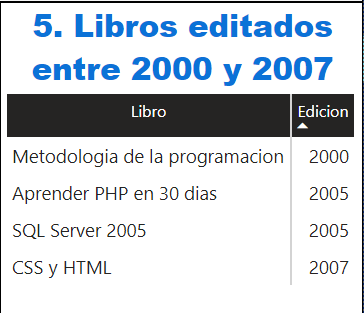
\includegraphics[width=13cm]{./img/img17.png}
        \end{center}
        \item Mostrar cuántos libros que se han prestado y agruparlos por el estante
        \begin{center}
            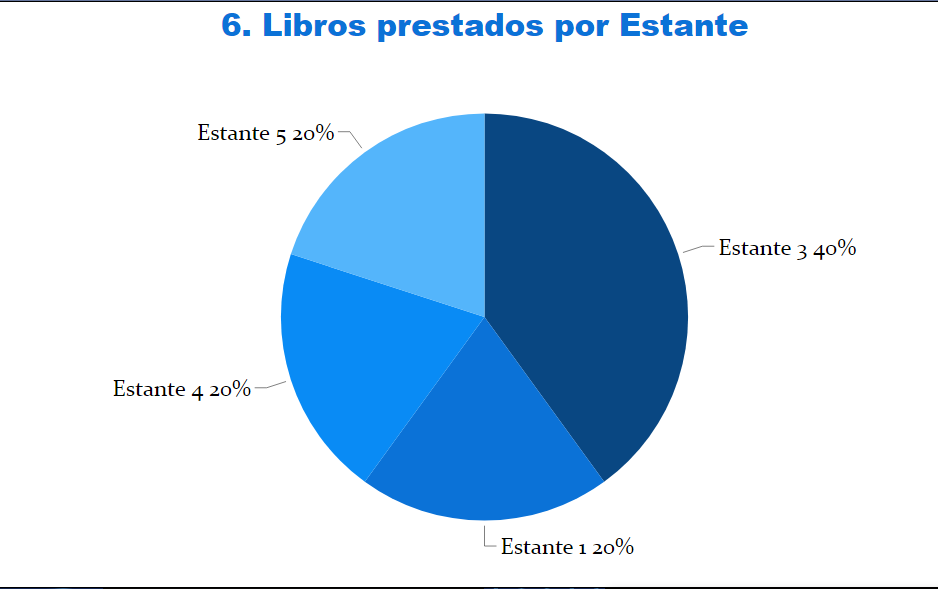
\includegraphics[width=13cm]{./img/img18.png}
        \end{center}
    \end{enumerate}
    Finalmente nuestro dashboard se veria de la siguiente manera con todos los reportes solicitados.
    \begin{center}
        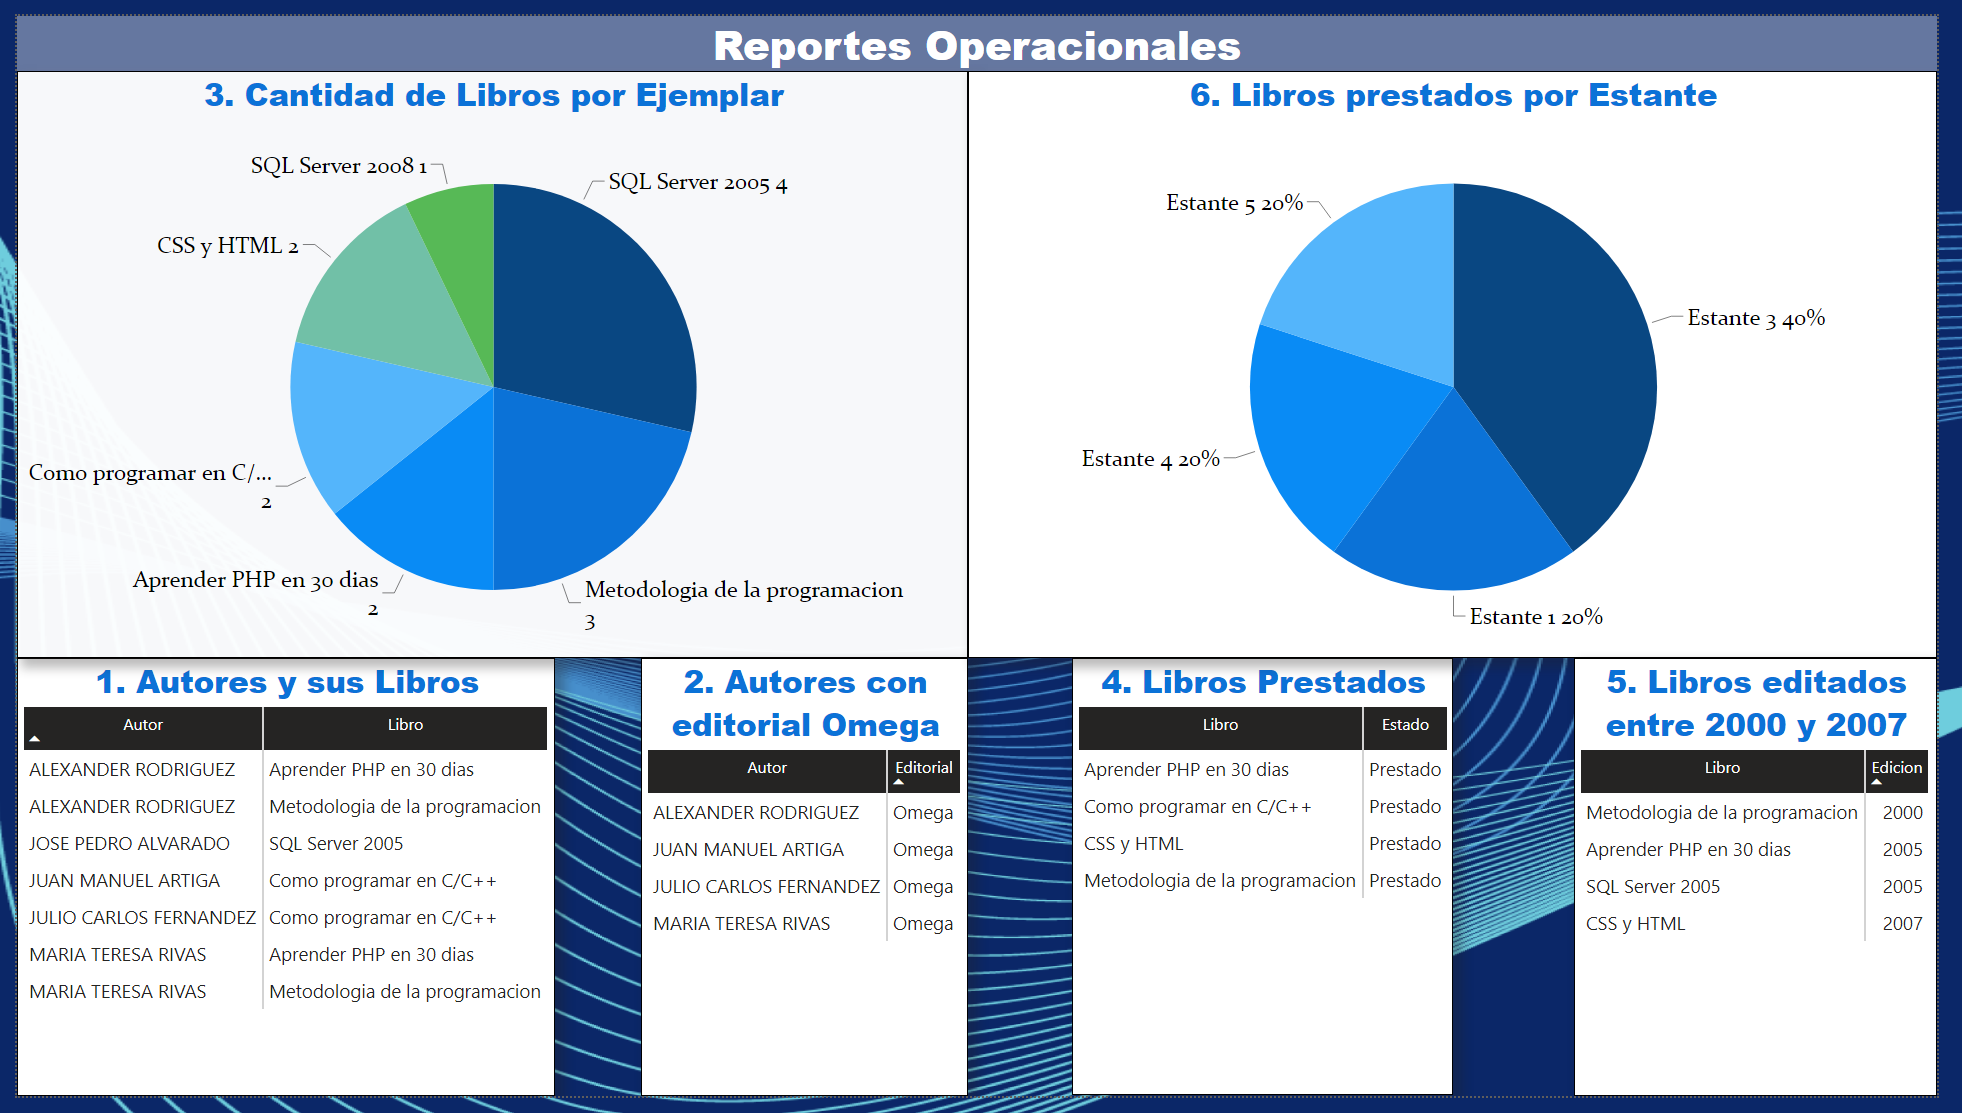
\includegraphics[width=18cm]{./img/img19.png}
    \end{center}
    %%%%%%%%%%%%%%%%%%%%%%%%%%%%%%%%%%%%%%%%%%%%%%%%%%%%%%%%%%%%%%%%%%%%%%%%%%%%%%%%%%%%%%%%%%%%%%%%%%%%%%%%%%%%%%%%%%%%%%%%%%%%%%%%%%%%%%%%%%%%%%%%%%%%%%%%%%%%%%%%%%%%%%%%%%%%%%%%%%%%%%%%%%%%%%%%%%%%%%%%%%%%%%%%%%%%%%%%%%%%%%%%%%%%%%%%%%%%%%%%%%%%%%%%%%%%%%%%%%%%%%%%%%%%%%%%%%%%%%%%%%%%%%%%%%%%%%%%%%%%%%%%%%%%%%%%%%%%%%%%%%%%%%%%%%%%%%%%%%%%%%%%%%%%%%%%%%%%%%%%%%%%%%%%%%%%%%%%%%%%%%%%%%%%%%%%%%%%%%%%%%%%%%%%%%%%%%%%%%%%%%%%%%%%%%%%%%%%%%%%%%%%%%%%%%%%%%%%%%%%%%%%%%%%%%%%%%%%%%%%%%%%%%%%%%%%%%%
    \newpage
    \section{CONCLUSIONES}
    \begin{itemize}
        \item Se logro crear correctamente los reportes operacionales de la misma manera que se hizo con Queries en SQL Server que en un Visualizador de datos, en este caso Power BI, obteniendo los mismos resultados en ambos casos, pero es obvio que es mucho más entendible los resultados que nos ofrece el Power BI a diferencia del SQL Server que pocas podrían comprender y también.
        \item Es mucho más sencillas elaborar los reportes en Power BI, ya que solo es cuestión de ir arrastrando los campos en los lugares que se crea necesaria de manera intuitiva a diferencia del SQL Server que se tiene que tener conocimiento básico para poder realizar las consultas.
    \end{itemize}
    %%%%%%%%%%%%%%%%%%%%%%%%%%%%%%%%%%%%%%%%%%%%%%%%%%%%%%%%%%%%%%%%%%%%%%%%%%%%%%%%%%%%%%%%%%%%%%%%%%%%%%%%%%%%%%%%%%%%%%%%%%%%%%%%%%%%%%%%%%%%%%%%%%%%%%%%%%%%%%%%%%%%%%%%%%%%%%%%%%%%%%%%%%%%%%%%%%%%%%%%%%%%%%%%%%%%%%%%%%%%%%%%%%%%%%%%%%%%%%%%%%%%%%%%%%%%%%%%%%%%%%%%%%%%%%%%%%%%%%%%%%%%%%%%%%%%%%%%%%%%%%%%%%%%%%%%%%%%%%%%%%%%%%%%%%%%%%%%%%%%%%%%%%%%%%%%%%%%%%%%%%%%%%%%%%%%%%%%%%%%%%%%%%%%%%%%%%%%%%%%%%%%%%%%%%%%%%%%%%%%%%%%%%%%%%%%%%%%%%%%%%%%%%%%%%%%%%%%%%%%%%%%%%%%%%%%%%%%%%%%%%%%%%%%%%%%%%%
    \newpage
    \section{WEBGRAFIA}
    \begin{itemize}
        \item GitHub. (2015). ExploraVisualizaconR.\\
        Recuperado de \textcolor{azul}{\url{https://github.com/fcharte/ExploraVisualizaconR}}
        \item Code Like a Girl. (2018). Análisis y visualización de datos con Pandas \& MatPlotLib.\\
        Recuperado de \textcolor{azul}{\url{https://code.likeagirl.io/analisis-y-visualizacion-de-datos-con-pandas-matplotlib-85ee4d7b4cad}}
        \item Analitics Lane. (2018). Visualización de datos en Python con Seaborn.\\
        Recuperado de \textcolor{azul}{\url{https://www.analyticslane.com/2018/07/20/visualizacion-de-datos-con-seaborn/}}
        \item Microdsosft Docs. (2020). Tutoial de Python: Explorar y visualizar datos.\\
        Recuperado de \textcolor{azul}{\url{https://docs.microsoft.com/es-es/sql/machine-learning/tutorials/python-taxi-classification-explore-data?view=sql-server-2017}}
        \item Hernández, A y Chacón, H. (2019). Manipulación, análisis y visualización de datos de la encuesta demográfica y de salud familiar con el programa R.\\
        Recuperado de \textcolor{azul}{\url{http://www.scielo.org.pe/scielo.php?script=sci_arttext&pid=S1726-46342019000100019&lng=es&nrm=iso&tlng=es}}
        \item GitHub. (2019). Analisis-Endes-Peru.\\
        Recuperado de \textcolor{azul}{\url{https://github.com/horaciochacon/Analisis-Endes-Peru}}
    \end{itemize}
\end{document}